\documentclass[10pt]{article}
% Layout matches the NeurIPS template (5.5in x 9in text block, Times).
% For submission: replace the next three lines with \usepackage{neurips_2026} (official style file).
\usepackage[letterpaper,textwidth=5.5in,textheight=9in,top=1in,headsep=0.25in]{geometry}
\usepackage{times}
\usepackage[T1]{fontenc}
\usepackage[utf8]{inputenc}
\usepackage{amsmath,amssymb,booktabs,graphicx,xcolor,microtype}
\usepackage[numbers,sort&compress]{natbib}
\usepackage[hidelinks]{hyperref}
\usepackage{tikz}
\usetikzlibrary{positioning,arrows.meta,fit,backgrounds,calc}
\usepackage{caption}
\captionsetup{font=small,labelfont=bf}
\definecolor{ink}{HTML}{52514E}
\definecolor{cblue}{HTML}{2A78D6}
\definecolor{corange}{HTML}{EB6834}
\definecolor{caqua}{HTML}{1BAF7A}
\newcommand{\bgpt}{BehaviorGPT}

\title{Too Normal to Be Human:\\ Probing a Behavioral Foundation Model for LLM-Agent Detection}
\author{E.~Baena\\ Northeastern University\\ \texttt{e.baena@northeastern.edu}}
\date{}

\begin{document}
\maketitle

\begin{abstract}
LLM agents now browse and buy on behalf of people. Whether a platform can tell them from their owners matters for fraud, account takeover, and in sensitive settings for insider-risk monitoring. A natural candidate is a \emph{behavioral foundation model}: a sequence model pretrained on billions of user actions whose next-action likelihood should flag anything that is not human.
We test this with \bgpt{} (12.5B parameters, 150B e-commerce actions), using its public API and its vendor's own anomaly-scoring method.
In a WebShop pilot, agents look \emph{less} surprising than humans, but we show that this is entirely a search-engine confound. Once the shown list is controlled, AUROC falls from 0.57 to 0.50.
We then introduce \emph{counterfactual replay} on OPeRA, a dataset of real Amazon sessions from 45 users. At each human click, an LLM agent acting for that user chooses from the identical result list with the identical history, so engine, query and context are fixed by construction.
Agents from two model families, with and without the user's persona, consistently choose items that \bgpt{} ranks \emph{higher} than the human's choice (paired $p\le 0.014$ in all three conditions): they are \emph{too normal}, not anomalous.
The signal is weak, however (step AUROC 0.54--0.58), and adds nothing to a five-feature logistic regression over the shown list (sponsored, position, rating, price, query overlap), which reaches 0.62--0.80.
Behavioral foundation models therefore need to be evaluated against cheap, context-matched baselines and under controlled engines, and anomaly-style detectors aimed at agents are pointed in the wrong direction.
\end{abstract}

\section{Introduction}
Web agents built on large language models (LLMs) can now search, compare and purchase on real sites \cite{yao2022webshop,deng2023mind2web,zhou2023webarena}. Increasingly they do so \emph{inside a human's account}, with the human's history, preferences and payment methods. For a platform, this raises a question that classic bot detection was not built for: given a real user's session, did the user or an agent acting for them make this choice? The same question arises wherever delegated agents operate on accounts that carry trust, from fraud and account takeover in commerce to insider-risk monitoring on government and defense networks.

Behavioral foundation models offer an attractive answer. Pretrained on very large logs of user actions, they assign a likelihood to every next action given a user's history, much as sequential recommenders do \cite{kang2018sasrec}. The vendor-recommended way to turn such a model into a detector is anomaly scoring: convert next-action scores into probabilities, compute excess surprisal, and accumulate it with a CUSUM statistic \cite{page1954cusum,unbox2026anomaly}. This assumes that non-human behavior is \emph{surprising}. LLM agents, however, are trained on human text and pick sensible, popular options. They may instead be \emph{too predictable}.

We test this assumption on \bgpt{} \cite{unbox2026docs} through its public API, at a total compute cost below US\$10. Our contributions are:
\begin{enumerate}
  \item \textbf{A confound.} In a WebShop pilot \cite{yao2022webshop}, agents appear less surprising than humans (AUROC 0.57), but the effect comes entirely from the search engine that produced each class's result lists. Measured within the shown list, it disappears (0.50; \S\ref{sec:pilot}).
  \item \textbf{A protocol.} \emph{Counterfactual replay} on real human sessions (OPeRA \cite{wang2025opera}): at every human click an agent chooses from the identical list with the identical history. Engine, query and context are held fixed by construction, and the setting matches delegated agents acting inside an account (\S\ref{sec:replay}).
  \item \textbf{A finding.} Across two model families and with or without the user's persona, agents are \emph{too normal}: \bgpt{} ranks their choices higher than the human's ($p\le0.014$). The signal is weak (AUROC 0.54--0.58) and redundant with five cheap list features, which reach 0.62--0.80 on their own (\S\ref{sec:results}).
\end{enumerate}
All code, prompts and cached API responses are released.

\paragraph{Related work.} LLM agents for web shopping are usually evaluated for task success \cite{yao2022webshop,deng2023mind2web,zhou2023webarena,zeng2023agenttuning}. A parallel line uses LLMs to \emph{simulate} human behavior \cite{park2023generative}, and OPeRA \cite{wang2025opera} was built to measure how well they imitate individual shoppers. We ask the converse, security-oriented question: can a model of human behavior tell them apart? The vendor's anomaly toolkit \cite{unbox2026anomaly} evaluates detection only on simulated perturbations. To our knowledge, this is the first evaluation of a behavioral foundation model against real LLM agents under a controlled engine.

\section{Setup}
\label{sec:setup}

\paragraph{The model.} \bgpt{}-v4 is a 12.5B-parameter sequence model trained on 150B e-commerce actions \cite{unbox2026docs}. Its API takes a user history (search, view, add-to-cart and order events) and, optionally, a query. It returns raw similarity scores for catalog items, not probabilities. A filter by item id scores any chosen set of items. We uploaded a private catalog of 74{,}347 products containing every item shown to or chosen by any human or agent in our data. In preliminary checks the API was deterministic, the history changed the ranking, and the model ignored timing below the hour. Because the API terms let the vendor train on uploaded content, we used only public data.

\paragraph{Scoring a choice in context.} For a choice $c$ made from a shown list $L$ (with $|L|=n$) after history $h$ and query $q$, one API call with the id filter set to $L$ gives scores $s_i(h,q)$ for all $i\in L$. We use:
\begin{itemize}
  \item the \textbf{within-list percentile} of $s_c$ in $L$ (1 means the model's top pick);
  \item the \textbf{conditional logit} $s_c/\tau-\log\sum_{i\in L}e^{s_i/\tau}+\log n$, with $\tau$ fit by maximum likelihood on human choices from the other half of the users (2-fold by user);
  \item the \textbf{history gain}: the percentile with $h$ minus the percentile with an empty history.
\end{itemize}
All three compare the choice only with what the chooser actually saw, so they are invariant to the engine that produced $L$. The vendor's original statistic instead compares $c$ against the whole catalog.

\paragraph{Baselines.} Five features of the chosen item within $L$, computed without \bgpt{}: log list position, sponsored flag, price percentile, star rating, and query--title word-overlap percentile. Detectors are logistic regressions on baselines, on \bgpt{} features, or on both, evaluated with 5-fold cross-validation grouped by user. We report AUROC with the agent as the positive class, with 95\% intervals from a bootstrap over users.

\section{Pilot: an engine confound}
\label{sec:pilot}
WebShop \cite{yao2022webshop} provides 1{,}643 human sessions on a 1.18M-product store. We took 150 test humans, plus 300 others to calibrate the vendor's statistic. We ran Claude Haiku 5.5 and DeepSeek V4 Flash on the same 150 instructions in a re-implementation of the store with BM25 search. With the vendor's method \cite{unbox2026anomaly}, agents look \emph{less} surprising (AUROC 0.57 for predictability, paired by instruction $p\approx0.001$, same sign for both models).

The effect is not behavioral. Our engine's lists were themselves more aligned with \bgpt{}: 63\% of their top-10 items fall in the model's top 100, against 56\% for the original engine. Scored within the list each chooser actually saw, the gap vanishes (AUROC 0.50 [0.44, 0.55], paired $p=0.59$; Fig.~\ref{fig:auroc}a). WebShop has two further problems: a median of one scored step per session, and instructed crowd workers who behave like agents by design. It is the wrong testbed.

\section{Counterfactual replay}
\label{sec:replay}

\begin{figure}[t]
\centering
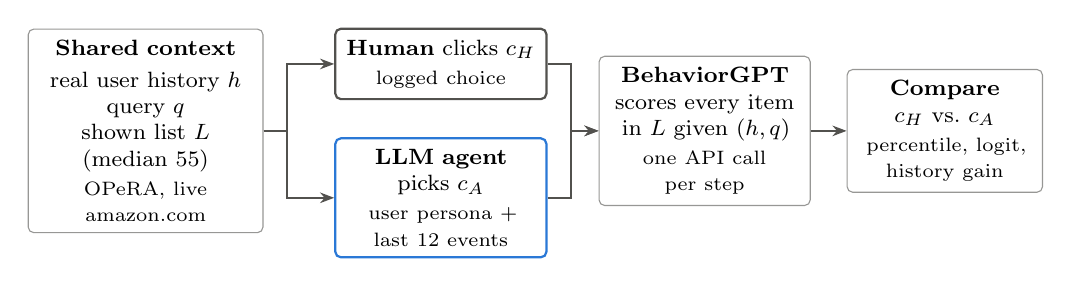
\begin{tikzpicture}[font=\footnotesize,
  box/.style={draw=ink!60, rounded corners=2pt, align=center, inner sep=4pt, fill=white, text width=#1},
  arr/.style={-{Stealth[length=1.8mm]}, ink, line width=0.6pt}]
\node[box=2.7cm] (ctx) at (0,0) {\textbf{Shared context}\\[2pt] real user history $h$\\ query $q$\\ shown list $L$ (median 55)\\[1pt]\scriptsize OPeRA, live amazon.com};
\node[box=2.4cm, draw=ink, line width=0.8pt] (hum) at (3.75,0.85) {\textbf{Human} clicks $c_H$\\[1pt]\scriptsize logged choice};
\node[box=2.4cm, draw=cblue, line width=0.8pt] (ag) at (3.75,-0.85) {\textbf{LLM agent} picks $c_A$\\[1pt]\scriptsize user persona + last 12 events};
\node[box=2.4cm] (bg) at (7.1,0) {\textbf{\bgpt{}}\\ scores every item in $L$ given $(h,q)$\\[1pt]\scriptsize one API call per step};
\node[box=2.2cm] (out) at (10.15,0) {\textbf{Compare} $c_H$ vs.\ $c_A$\\[1pt]\scriptsize percentile, logit, history gain};
\draw[arr] (ctx.east) -- ++(0.3,0) |- (hum.west);
\draw[arr] (ctx.east) -- ++(0.3,0) |- (ag.west);
\draw[arr] (hum.east) -- ++(0.3,0) |- (bg.west);
\draw[arr] (ag.east) -- ++(0.3,0) |- (bg.west);
\draw[arr] (bg.east) -- (out.west);
\end{tikzpicture}
\caption{\textbf{Counterfactual replay.} At each human click, an agent acting for the same user chooses from the identical list with the identical history. Engine, query and context are held fixed, so any difference between the two choices comes from the chooser.}
\label{fig:design}
\end{figure}

\paragraph{Human data.} OPeRA \cite{wang2025opera} logs real users shopping on Amazon with a browser plug-in, along with their self-reported personas. From the full release (54 users, 692 sessions) we build one time-ordered event stream per user across all of that user's sessions. We extract every click on a product in a search-result list where the logged page contains the full list. This gives 384 steps from 45 users, with a median list size of 55 and a median of 13 history events per API call.

\paragraph{Agents.} At each step, an LLM receives the user's survey persona, their last 12 events, the query and the full list in page order (title, price, rating, sponsored flag), and returns the item it would open (Fig.~\ref{fig:design}). There are three conditions: Claude Haiku 5.5 with persona, the same without persona, and DeepSeek V4 Flash with persona (temperature 0.7). Haiku answered every step. DeepSeek answered 247 of 384 validly; the remaining responses were empty or malformed. Agents chose the same item as the human in 10\%, 14\% and 19\% of steps, respectively.

\paragraph{Why this design.} It removes the two confounds that undermine naive comparisons: the engine (both choices come from one list) and the intent (both act on the same query and history). It also matches the threat model of a delegated agent operating within a legitimate account. The cost is that each decision is judged in isolation; we return to this in \S\ref{sec:discussion}.

\section{Results}
\label{sec:results}

\begin{figure}[t]
\centering
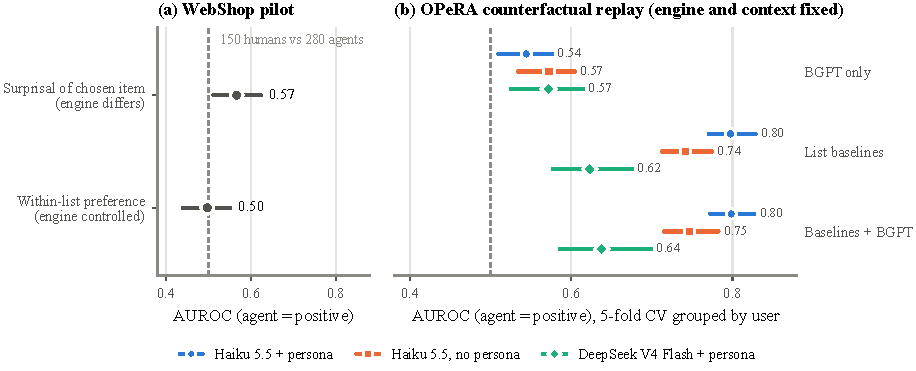
\includegraphics[width=\linewidth]{figures/fig_auroc.pdf}
\caption{\textbf{Detection performance with 95\% user-cluster bootstrap intervals.} (a) In the WebShop pilot, the apparent signal (agents less surprising) disappears once choices are scored within the list each chooser saw. (b) In counterfactual replay, \bgpt{} alone detects agents only weakly. Five list features detect them far better, and adding \bgpt{} to them changes AUROC by at most 0.015.}
\label{fig:auroc}
\end{figure}

\paragraph{Agents are too normal.} With engine and context fixed, all three agent conditions choose items that \bgpt{} ranks higher than the human's choice (Fig.~\ref{fig:shift}; Table~\ref{tab:main}). The mean within-list percentile rises from 0.59 to 0.64--0.67. The effect is significant in every condition (paired Wilcoxon $p=0.014$, $3.3\times10^{-5}$ and $2.6\times10^{-4}$) and holds for the conditional logit. This is the opposite of the assumption behind anomaly scoring: an agent operating inside an account makes the account look \emph{more} typical, not less, so a CUSUM on excess surprisal would drift away from an alarm.

\begin{figure}[t]
\centering
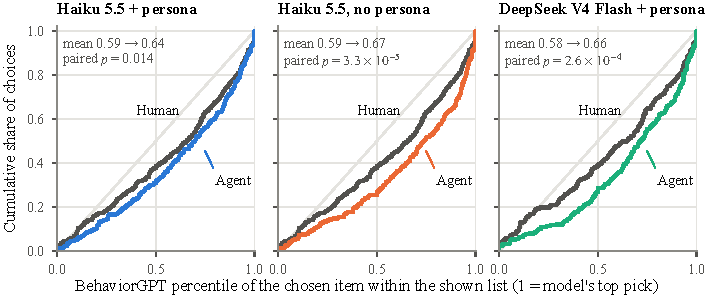
\includegraphics[width=\linewidth]{figures/fig_shift.pdf}
\caption{\textbf{Agents pick what the model expects.} Cumulative distribution of the \bgpt{} within-list percentile of the chosen item. Curves further to the right mean more model-typical choices. Human and agent choices are paired by step; $p$ from a paired Wilcoxon test.}
\label{fig:shift}
\end{figure}

\begin{table}[t]
\centering
\small
\caption{\textbf{\bgpt{} statistics, human vs.\ agent on identical context.} Means, paired Wilcoxon $p$, and AUROC at the step level (user-cluster bootstrap CI) and at the user level (per-user means, 45 vs.\ 45).}
\label{tab:main}
\setlength{\tabcolsep}{3.5pt}
\begin{tabular}{llcccc}
\toprule
Agent & Statistic & Human / Agent & Paired $p$ & Step AUROC & User AUROC \\
\midrule
Haiku 5.5 + persona & percentile & 0.590 / 0.635 & 0.014 & 0.54 [0.51, 0.58] & 0.61 \\
 & logit & 0.068 / 0.111 & 0.032 & 0.54 [0.50, 0.57] & 0.59 \\
 & history gain & 0.021 / 0.043 & 0.012 & 0.55 [0.51, 0.59] & 0.58 \\
\addlinespace
Haiku 5.5, no pers.\ & percentile & 0.590 / 0.670 & $3.3\times10^{-5}$ & 0.58 [0.54, 0.61] & 0.65 \\
 & logit & 0.068 / 0.156 & $1.5\times10^{-4}$ & 0.57 [0.54, 0.61] & 0.64 \\
 & history gain & 0.021 / 0.048 & 0.004 & 0.54 [0.50, 0.59] & 0.59 \\
\addlinespace
DeepSeek V4 Flash & percentile & 0.578 / 0.665 & $2.6\times10^{-4}$ & 0.58 [0.52, 0.63] & 0.62 \\
 & logit & 0.048 / 0.151 & $8.1\times10^{-4}$ & 0.57 [0.53, 0.63] & 0.61 \\
 & history gain & 0.001 / 0.029 & 0.019 & 0.55 [0.50, 0.59] & 0.58 \\
\bottomrule
\end{tabular}
\end{table}

\paragraph{But the signal is weak and redundant.} On its own, \bgpt{} reaches a step AUROC of 0.54--0.58, and 0.61--0.65 when averaged per user (Fig.~\ref{fig:auroc}b). The five list features alone reach 0.80 (Haiku with persona), 0.74 (Haiku without persona) and 0.62 (DeepSeek). Adding \bgpt{} changes these by $+0.001$, $+0.005$ and $+0.015$, all well inside the confidence intervals. The ROC curves for baselines and baselines + \bgpt{} overlap almost everywhere (Fig.~\ref{fig:roc}).

\paragraph{What gives agents away.} The cheap tells are behavioral, not semantic (Fig.~\ref{fig:tells}). Humans click a sponsored result in 34\% of steps, against 5\% for Haiku with persona and 23\% for DeepSeek. Haiku also reads deeper into the list (mean rank 18 vs.\ 8). All agents pick items with higher star ratings and more literal query matches. The last tell partly explains the \bgpt{} effect: given a query, the model favors on-topic, popular items, and so do agents.

\begin{figure}[t]
\centering
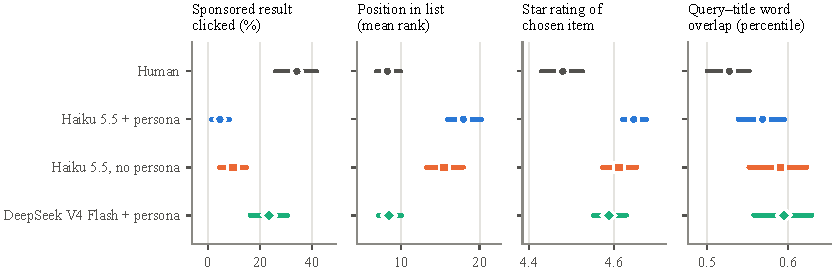
\includegraphics[width=\linewidth]{figures/fig_tells.pdf}
\caption{\textbf{Cheap tells.} Properties of the chosen item for humans and agents on the same 384 steps (247 for DeepSeek). Means with 95\% user-cluster bootstrap intervals. Agents avoid ads, prefer highly rated and literally matching items, and Haiku scrolls further down the list.}
\label{fig:tells}
\end{figure}

\paragraph{History and persona.} Conditioning on the user's history raises the percentile of human choices only from 0.569 to 0.590. In other words, the user's past actions add little predictive power for which listed item a person opens. For agents, history helps \emph{more} (history gain 0.03--0.05 vs.\ 0.00--0.02), probably because agents see the recent events in their prompt and stay consistent with them. Giving the agent the user's persona does not make it harder for \bgpt{} to detect (step AUROC 0.54 vs.\ 0.58 without persona; the intervals overlap). It does change its style: without the persona Haiku clicks more ads and stays higher in the list, which lowers the baseline detector from 0.80 to 0.74. The model family matters more than the persona: DeepSeek is the hardest agent to detect by any method.

\begin{figure}[t]
\centering
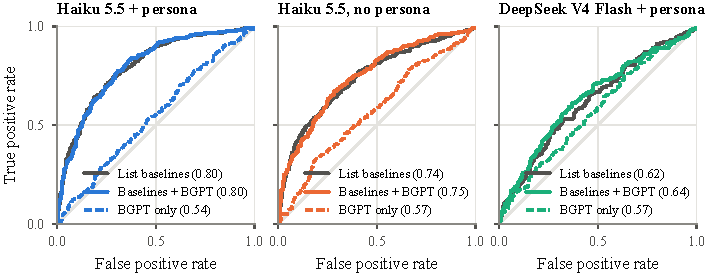
\includegraphics[width=\linewidth]{figures/fig_roc.pdf}
\caption{\textbf{ROC curves} for the three detectors (5-fold CV grouped by user; AUROC in parentheses). Adding \bgpt{} to the list baselines (solid colored line) barely moves the baseline curve (gray).}
\label{fig:roc}
\end{figure}

\section{Whole trajectories under the original engine}
\label{sec:traj}

Counterfactual replay judges single decisions. Agents may give themselves away more clearly in \emph{how} they shop: how many products they compare, whether they go back, how they search. We test this on WebShop, the one setting where both classes can produce complete sessions in the same environment.

\paragraph{Setup.} We rebuilt WebShop's original search engine (pyserini 0.17 BM25 over the full catalog of 1.18M products). For 99.6\% of 2{,}364 human searches it reproduces the logged first results page exactly, so the engine confound of \S\ref{sec:pilot} is removed. Claude Haiku 5.5 and DeepSeek V4 Flash then shopped in the official WebShop text environment. They had the humans' action space (search, paginate, open product, choose options, read sub-pages, buy) and up to 20 steps per episode. Their goals were the same 150 instructions as the test humans, with each human's target product and price limit. This gives 150 human--agent pairs per model.

We compute 14 trajectory features with one function for both classes:
\begin{itemize}
  \item pages visited, queries and reformulations, query length and overlap with the instruction;
  \item products viewed, deepest results page, sub-pages, option clicks, returns to the results list;
  \item purchase, and the rank of the purchased item.
\end{itemize}
\bgpt{} scores each session with the vendor method: mean excess surprisal, its $z$-score, mean log-rank, and one-sided CUSUM statistics in both directions (``surprising'' and ``too normal''). Calibration uses human sessions from the other fold. Detectors use 5-fold cross-validation grouped by instruction pair.

\begin{figure}[t]
\centering
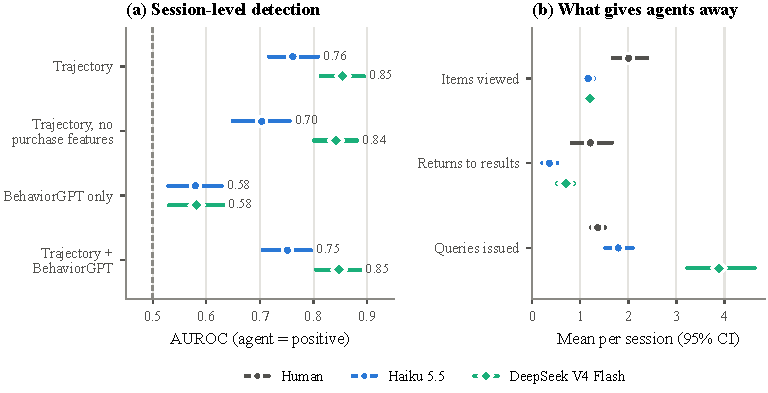
\includegraphics[width=\linewidth]{figures/fig_traj.pdf}
\caption{\textbf{Whole trajectories, same engine.} (a) Session-level AUROC with 95\% pair-bootstrap intervals. Trajectory features detect both agents. The control without purchase features addresses the fact that every human demonstration ends in a purchase. \bgpt{} alone stays near 0.58 and adds nothing when combined. (b) Haiku compares few products and rarely goes back to the results; DeepSeek over-searches.}
\label{fig:traj}
\end{figure}

\paragraph{Results.} Trajectory features separate humans from agents well: AUROC 0.76 [0.72, 0.81] for Haiku and 0.85 [0.81, 0.89] for DeepSeek (Fig.~\ref{fig:traj}a). Every human demonstration ends in a purchase, whereas agents sometimes stop without buying. To rule this out as the source of the signal, we dropped the purchase-related features (0.70 and 0.84) and also kept only pairs in which the agent bought (0.66 and 0.81). Both checks leave the trajectory detector well above \bgpt{}, which reaches 0.58 for both agents on its own and lowers the combined detector slightly (by 0.01 for both agents).

The two agents are caught in different ways (Fig.~\ref{fig:traj}b). Haiku hardly comparison-shops: it views 1.2 products per session against 2.0 for humans and returns to the results list 0.35 times against 1.2. DeepSeek over-searches, issuing 3.9 queries per session against 1.4 for humans, and shorter ones (5.8 vs.\ 6.7 words). On the \bgpt{} side, agent sessions are again slightly \emph{less} surprising than human ones (mean excess surprisal 0.02 for Haiku and 0.08 for DeepSeek, against 0.10 for humans), but the difference does not separate the classes.

\paragraph{Why the foundation model misses it.} \bgpt{} scores \emph{which product} is chosen next. A WebShop session yields a median of one scored step, and the behaviors that separate the classes (comparing, backtracking, reformulating) are navigation, which a next-item model does not score. Timing could add further signal, but the model ignores time below the hour.

\section{Discussion}
\label{sec:discussion}

\paragraph{Implications for detection.} The vendor's anomaly pipeline flags behavior the model finds surprising. Against LLM agents this points the wrong way: at the level of single choices, agents are slightly \emph{more} typical than the humans they act for. A detector built on a behavioral foundation model would need a two-sided or ``too-typical'' test. Even then it would add nothing over a handful of list features that any platform already logs. Advertising engagement in particular is a strong, cheap and so far overlooked signal of a human chooser.

\paragraph{Implications for evaluation.} Our pilot shows how easily a spurious effect appears: a different search engine alone produced a significant, model-consistent difference between humans and agents. Any comparison of humans and agents across environments, including agent benchmarks that reuse human demonstrations \cite{yao2022webshop,zeng2023agenttuning}, should score choices relative to what each chooser was shown. Counterfactual replay on logged human sessions does this by construction and is cheap: about 1{,}000 LLM calls and 768 API calls here.

\paragraph{Limitations.} We judge single decisions, not whole agent sessions, so query formulation, navigation, timing and dwell, plausibly the strongest agent tells, are out of scope. \bgpt{} cannot read them anyway, since it ignores time below the hour. OPeRA products enter the catalog with title and price only, which may weaken the model's item representations. DeepSeek's 36\% invalid responses may select easier steps. Our sample of 45 users is small for user-level claims. We test one behavioral foundation model through its public interface, without access to its weights.

\paragraph{Broader impact.} Detection of delegated agents can protect users and platforms. It can also be used to block legitimate assistive agents, and our findings suggest that crude heuristics (ad avoidance) would do so with many false positives. For sensitive deployments such as defense or government networks, current hosted behavioral models are unsuitable regardless of accuracy, because their terms allow training on uploaded data. We used only public datasets.

\section{Conclusion}
A behavioral foundation model can tell LLM agents from the humans they act for, but only weakly, in the opposite direction to the one anomaly detection assumes, and not beyond what five cheap features already provide. Engine-controlled, context-matched evaluation, here through counterfactual replay, is necessary to see this; without it, a search-engine confound produces a convincing but spurious effect.


\bibliographystyle{plainnat}
\bibliography{refs}

\end{document}
